\documentclass[10pt,conference,a4paper]{article}

% ─────────────────────────── encoding & language
\usepackage[T1]{fontenc}
\usepackage[utf8]{inputenc}
\usepackage[provide=*,indonesian]{babel}

% ─────────────────────────── page layout (two-column academic)
\usepackage[a4paper,margin=2cm]{geometry}

% ─────────────────────────── typography
\usepackage{lmodern}
\usepackage{microtype}
\usepackage{parskip}
\renewcommand{\baselinestretch}{1.05}

% ─────────────────────────── math, tables, figures
\usepackage{amsmath,amssymb}
\usepackage{graphicx}
\usepackage{booktabs}
\usepackage{caption}
\usepackage{subcaption}
\usepackage{float}
\usepackage{array}
\usepackage{tabularx}
\usepackage{makecell}

% ─────────────────────────── code listings
\usepackage{listings}
\usepackage{xcolor}
\definecolor{codegray}{rgb}{0.95,0.95,0.95}
\definecolor{codeblue}{rgb}{0.16,0.36,0.55}
\definecolor{codegreen}{rgb}{0.0,0.5,0.0}
\lstdefinestyle{pystyle}{
  backgroundcolor=\color{codegray},
  basicstyle=\ttfamily\footnotesize,
  keywordstyle=\color{codeblue}\bfseries,
  commentstyle=\color{codegreen}\itshape,
  stringstyle=\color{codeblue},
  language=Python,
  breaklines=true,
  showstringspaces=false,
  frame=single,
  framerule=0pt,
  xleftmargin=4pt,
  xrightmargin=4pt,
}
\lstset{style=pystyle}

% ─────────────────────────── hyperlinks
\usepackage[hidelinks,colorlinks=true,linkcolor=black,urlcolor=blue!60!black,citecolor=blue!60!black]{hyperref}
\usepackage{url}

% ─────────────────────────── title styling
\usepackage{titling}
\setlength{\droptitle}{-1.2cm}

\title{\vspace{-0.4cm}\bfseries\Large
  Implementasi dan Analisis Komparatif Transformer pada Klasifikasi Teks, Vision Transformer, serta Super-Resolution Gambar
}

\author{
  Firmansyah Sundana\thanks{Email: sundana@student.ub.ac.id}\\
  \textit{NIM: 257150100011009}\\
  \textit{Mata Kuliah: Topik Pembelajaran Mesin}
}
\date{12 Mei 2026}

\begin{document}

\maketitle
\begin{abstract}
  \noindent\textbf{Abstrak.}
  Laporan ini menyajikan implementasi \emph{from-scratch} arsitektur Transformer pada tiga domain: (i) klasifikasi sentimen teks pada dataset IMDb (50K review), (ii) klasifikasi gambar pada CIFAR-10 menggunakan Vision Transformer (ViT), dan (iii) tugas non-klasifikasi berupa \emph{Single Image Super-Resolution} menggunakan model Swin2SR yang telah dilatih sebelumnya (\emph{pretrained}). Hasil eksperimen menunjukkan bahwa Transformer tidak selalu unggul: pada IMDb, Transformer hanya unggul tipis (87{,}51\%) dibandingkan MLP sederhana (87{,}03\%), sementara pada CIFAR-10, SmallResNet (76{,}17\%) mengungguli ViT (66{,}03\%) sebesar 9{,}5 poin persentase dengan jumlah parameter $\sim$3$\times$ lebih sedikit. Pengaruh hiperparameter struktural (panjang sekuens, ukuran \emph{patch}) terhadap akurasi diukur dan dianalisis. Selanjutnya, dilakukan modifikasi terhadap kode Swin2SR berupa \emph{tiled inference} dengan \emph{feathered blending} untuk mendukung gambar berukuran sembarang tanpa OOM (\emph{Out-Of-Memory}); validasi menunjukkan output identik dengan inferensi biasa (rata-rata selisih piksel $\approx 0{,}05\%$). Studi ini menegaskan bahwa \emph{inductive bias} arsitektur konvolusional masih relevan pada dataset kecil, sementara Transformer memerlukan data masif atau \emph{pretraining} untuk mencapai potensi penuhnya.

  \medskip
  \noindent\textit{Kata kunci---}\,Transformer, Vision Transformer, Klasifikasi Teks, IMDb, CIFAR-10, Super-Resolution, Swin2SR, \emph{Tiled Inference}.
\end{abstract}

% ════════════════════════════════════════════════════════════════════
\section{Pendahuluan}
% ════════════════════════════════════════════════════════════════════

Arsitektur Transformer \cite{vaswani2017} merupakan tulang punggung model modern di bidang \emph{natural language processing}, \emph{computer vision}, dan \emph{multimodal learning}. Mekanisme \emph{self-attention} yang ditawarkan memungkinkan model menangkap dependensi jarak jauh tanpa terkendala oleh rekurensi atau lokalitas konvolusi.

Meskipun demikian, klaim superioritas Transformer perlu diuji pada konteks yang adil: ketika data terbatas atau tugas didominasi oleh pola lokal, model dengan \emph{inductive bias} yang sesuai (CNN, LSTM) sering kali kompetitif atau bahkan unggul \cite{dosovitskiy2021}.

Laporan ini mendokumentasikan eksperimen komparatif pada tiga domain:
\begin{enumerate}\itemsep0pt
  \item \textbf{Klasifikasi Teks} — TransformerEncoder vs. MLP, CNN-1D \cite{kim2014}, dan RNN bidirectional pada IMDb 50K \cite{maas2011}.
  \item \textbf{Klasifikasi Gambar} — Vision Transformer (ViT) \cite{dosovitskiy2021} vs. MLP gambar, SimpleCNN, dan SmallResNet \cite{he2016} pada CIFAR-10 \cite{krizhevsky2009}.
  \item \textbf{Super-Resolution} — implementasi inference dan modifikasi (\emph{tiled inference}) pada Swin2SR \cite{conde2022,liang2021}.
\end{enumerate}

Tujuan utama tugas ini bukan mengejar akurasi tertinggi, melainkan memahami implementasi, mengukur \emph{trade-off}, dan membaca/memodifikasi kode \emph{open-source} nyata.

% ════════════════════════════════════════════════════════════════════
\section{Dataset}
% ════════════════════════════════════════════════════════════════════

\subsection{IMDb Movie Reviews (Text)}
Dataset IMDb \cite{maas2011} berisi 50.000 review film berbahasa Inggris dengan label biner (\emph{positive}/\emph{negative}); kelas seimbang sempurna 25k/25k. Pembagian \emph{train}/\emph{test} 80/20 dilakukan secara \emph{stratified} dengan \texttt{random\_state=42}. Distribusi panjang review ditunjukkan pada Gambar~\ref{fig:imdb-dist}; median $\approx 173$ kata dan persentil ke-90 sekitar 357 kata, menjadi dasar pemilihan \texttt{max\_len=256} untuk eksperimen utama.

\begin{figure}[H]
  \centering
  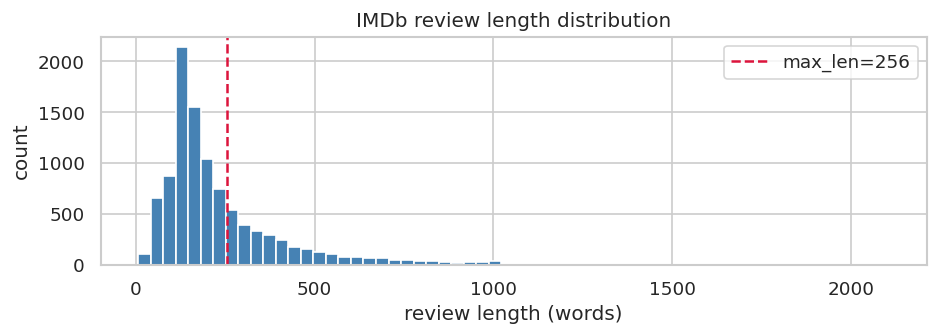
\includegraphics[width=\linewidth]{figures/imdb_length_distribution.png}
  \caption{Distribusi panjang review IMDb (dalam jumlah kata). Garis merah putus-putus menandai batas pemotongan $\texttt{max\_len}=256$.}
  \label{fig:imdb-dist}
\end{figure}

\subsection{CIFAR-10 (Vision)}
CIFAR-10 \cite{krizhevsky2009} terdiri dari 60.000 gambar berwarna $32\times32$ piksel dalam 10 kelas (50k \emph{train}, 10k \emph{test}). Augmentasi yang digunakan pada training: \texttt{RandomCrop(32, padding=4)} dan \texttt{RandomHorizontalFlip}, diikuti normalisasi dengan rata-rata dan deviasi standar kanonik. Contoh sampel ditampilkan pada Gambar~\ref{fig:cifar-samples}.

\begin{figure}[H]
  \centering
  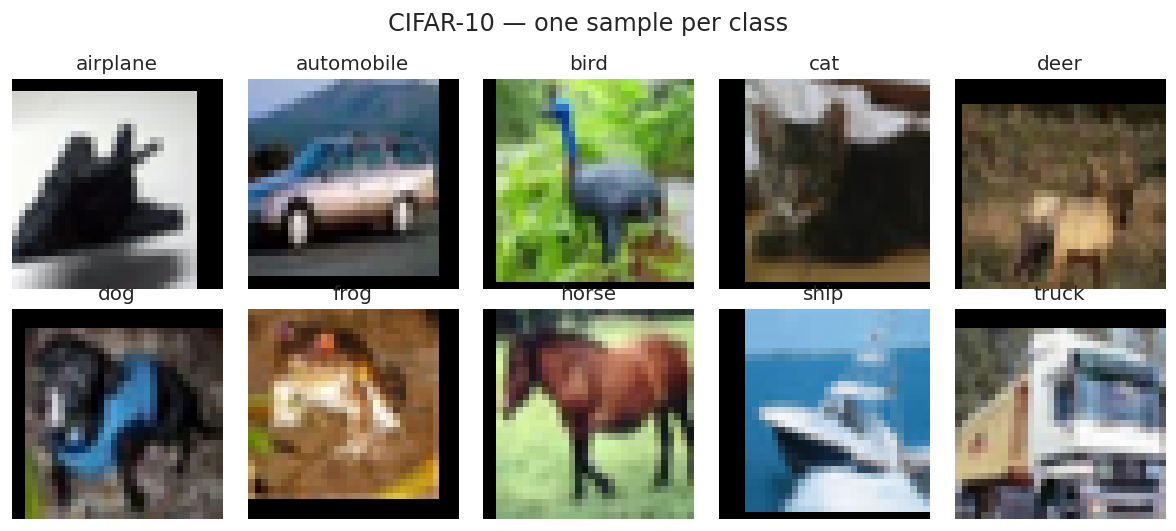
\includegraphics[width=\linewidth]{figures/cifar10_samples.png}
  \caption{Satu contoh sampel untuk setiap kelas CIFAR-10.}
  \label{fig:cifar-samples}
\end{figure}

% ════════════════════════════════════════════════════════════════════
\section{Arsitektur Model}
% ════════════════════════════════════════════════════════════════════

Seluruh blok Transformer dan ViT ditulis \emph{dari nol} di PyTorch (tanpa \texttt{nn.TransformerEncoder} bawaan), untuk memastikan pemahaman penuh atas alurnya.

\subsection{Model Teks}
Setiap model menerima sekuens token \texttt{(B, T)} dan menghasilkan \emph{logits} \texttt{(B, 2)}.

\begin{itemize}\itemsep1pt
  \item \textbf{TransformerClassifier}: Embedding + \emph{Sinusoidal Positional Encoding} + 2$\times$ TransformerEncoderBlock (MultiHeadAttention + FFN + LayerNorm) + \emph{mean-pooling} mengabaikan padding + Linear. \\
  Konfigurasi: $d_{\text{model}}{=}128$, $h{=}4$, $L{=}2$, $d_{\text{ff}}{=}256$, \emph{dropout}~0{,}1.

  \item \textbf{MLPClassifier}: Embedding $\rightarrow$ \emph{mean-pool} $\rightarrow$ FC$[256, 128]$ $\rightarrow$ Linear. Baseline paling sederhana namun mengejutkan kuat untuk sentimen.

  \item \textbf{CNN1DClassifier} (TextCNN \cite{kim2014}): Embedding $\rightarrow$ \emph{parallel} Conv1d kernel size $\{2,3,4\}$ + ReLU + \emph{max-over-time pooling} + dropout + Linear.

  \item \textbf{RNNClassifier}: Embedding $\rightarrow$ 2-layer biRNN $\rightarrow$ \emph{last hidden state} + Linear.
\end{itemize}

\subsection{Model Gambar (CIFAR-10)}

\begin{itemize}\itemsep1pt
  \item \textbf{ViT}: PatchEmbedding (\texttt{Conv2d} $4{\times}4$, \emph{stride}~4 $\Rightarrow$ 64 \emph{patches}) + token \texttt{[CLS]} + \emph{learnable positional embedding} + 6$\times$ TransformerEncoderBlock (di-import dari \texttt{models/transformer.py}, tidak duplikat) + LayerNorm + Linear pada token \texttt{[CLS]}. $d_{\text{model}}{=}192$, $h{=}6$, $L{=}6$, $d_{\text{ff}}{=}384$.

  \item \textbf{ImageMLP}: \emph{Flatten} $3\cdot32\cdot32$ + FC$[512, 256]$ + Dropout.

  \item \textbf{SimpleCNN}: 3 blok Conv-BN-ReLU-Pool (32$\rightarrow$64$\rightarrow$128) + \emph{Global Average Pooling}. Sangat ringan (95k parameter).

  \item \textbf{SmallResNet}: Stem + 3 \emph{stage} ResNet (32$\rightarrow$64$\rightarrow$128), 6 BasicBlock, implementasi sendiri (bukan torchvision).
\end{itemize}

\subsection{Konfigurasi Training}
Untuk perbandingan adil, seluruh model menggunakan:
\begin{itemize}\itemsep0pt
  \item Optimizer Adam (lr$=10^{-3}$, weight\_decay$=10^{-5}$),
  \item Loss CrossEntropyLoss,
  \item 10 \emph{epoch}, batch $64$ (teks) atau $128$ (gambar),
  \item Random seed $42$ pada PyTorch dan CUDA.
\end{itemize}
Perangkat keras: NVIDIA RTX 5060 Ti, 17{,}1~GB VRAM, PyTorch 2.11 + CUDA 13.

% ════════════════════════════════════════════════════════════════════
\section{Hasil Eksperimen}
% ════════════════════════════════════════════════════════════════════

\subsection{Hasil Utama (10 epoch)}

Tabel~\ref{tab:summary} merangkum metrik akhir seluruh model. Kurva \emph{training/test loss} dan \emph{accuracy} ditampilkan pada Gambar~\ref{fig:text-curves} dan Gambar~\ref{fig:vision-curves}.

\begin{table*}[ht]
  \centering
  \caption{Hasil eksperimen utama text (IMDb) dan vision (CIFAR-10), 10 epoch.}
  \label{tab:summary}
  \small
  \begin{tabular}{l l c c r r r}
    \toprule
    \textbf{Model} & \textbf{Dataset} & \textbf{Accuracy} & \textbf{Loss} & \textbf{Parameter} & \textbf{Train Time} & \textbf{Inference/batch} \\
    \midrule
    \textbf{Transformer} & IMDb     & \textbf{0{,}8751} & 0{,}4827 & 2{.}841{.}730 & 120{,}7 s  &  5{,}68 ms \\
    MLP                  & IMDb     & 0{,}8703          & 0{,}5968 & 2{.}626{.}178 &  13{,}9 s  &  0{,}46 ms \\
    CNN1D                & IMDb     & 0{,}8682          & 0{,}6280 & 2{.}708{.}610 &  23{,}6 s  &  0{,}83 ms \\
    RNN                  & IMDb     & 0{,}7723          & 0{,}5342 & 2{.}725{.}378 &  26{,}8 s  &  0{,}84 ms \\
    \midrule
    ViT                  & CIFAR-10 & 0{,}6603          & 0{,}9684 & 1{.}806{.}538 & 134{,}1 s  & 10{,}58 ms \\
    ImageMLP             & CIFAR-10 & 0{,}4003          & 1{,}6271 & 1{.}707{.}274 &  60{,}7 s  &  8{,}20 ms \\
    SimpleCNN            & CIFAR-10 & 0{,}6151          & 1{,}1253 &    \textbf{94{.}986} &  69{,}4 s  &  9{,}05 ms \\
    \textbf{SmallResNet} & CIFAR-10 & \textbf{0{,}7617} & 0{,}7594 &   696{.}618   & 114{,}7 s  &  8{,}62 ms \\
    \bottomrule
  \end{tabular}
\end{table*}

\begin{figure}[H]
  \centering
  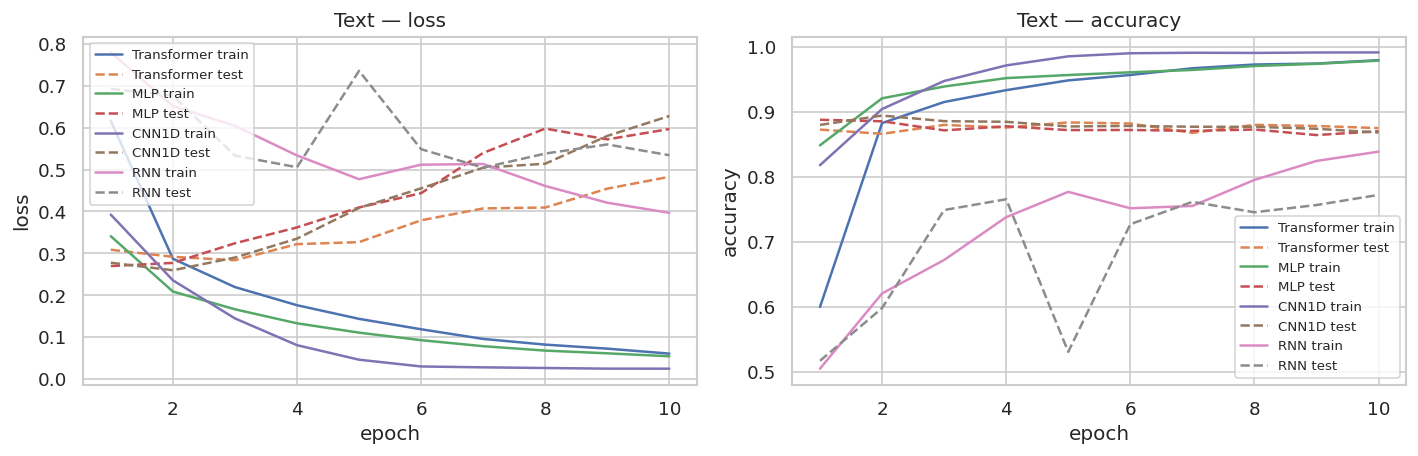
\includegraphics[width=\linewidth]{figures/text_training_curves.png}
  \caption{Kurva \emph{loss} dan \emph{accuracy} model teks pada IMDb (10 epoch). Garis solid: \emph{train}, putus-putus: \emph{test}.}
  \label{fig:text-curves}
\end{figure}

\begin{figure}[H]
  \centering
  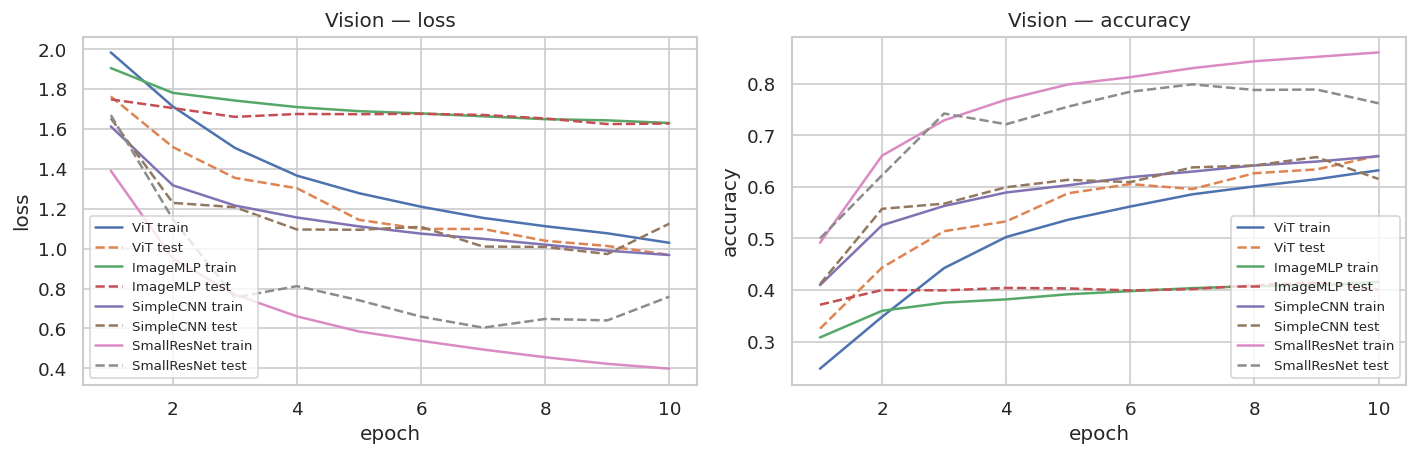
\includegraphics[width=\linewidth]{figures/vision_training_curves.png}
  \caption{Kurva \emph{loss} dan \emph{accuracy} model vision pada CIFAR-10.}
  \label{fig:vision-curves}
\end{figure}

\subsection{Eksperimen Variasi Hiperparameter}

\subsubsection{Variasi Sequence Length (Transformer/IMDb)}
Model Transformer dilatih ulang selama 5 epoch dengan \texttt{max\_len}\,$\in\{64, 128, 256, 512\}$ (Tabel~\ref{tab:seqlen}, Gambar~\ref{fig:variations}-kiri). Hasil menunjukkan peningkatan monoton hingga $L{=}256$; kenaikan dari 256 ke 512 hanya $+0{,}55$~pp namun memerlukan waktu 3$\times$ lebih besar, sesuai \emph{diminishing returns} setelah median panjang review tercapai.

\begin{table}[H]
  \centering
  \caption{Variasi \texttt{max\_len} pada Transformer/IMDb (5 epoch).}
  \label{tab:seqlen}
  \small
  \begin{tabular}{c c c}
    \toprule
    \texttt{max\_len} & Accuracy & Train Time \\
    \midrule
    64                  & 0{,}8078 & 18{,}8 s \\
    128                 & 0{,}8469 & 21{,}5 s \\
    \textbf{256}        & \textbf{0{,}8877} & 60{,}3 s \\
    512                 & 0{,}8932 & 192{,}4 s \\
    \bottomrule
  \end{tabular}
\end{table}

\subsubsection{Variasi Patch Size (ViT/CIFAR-10)}
ViT dilatih ulang dengan \texttt{patch\_size}\,$\in\{2,4,8,16\}$ (Tabel~\ref{tab:patch}, Gambar~\ref{fig:variations}-kanan). Patch kecil $p{=}2$ (256 patch) memberi akurasi terbaik namun 5$\times$ lebih mahal. Patch terlalu besar ($p{\geq}8$) menghancurkan konten spasial: pada $p{=}16$ hanya tersisa 4 patch, akurasinya jatuh ke 31{,}1\%.

\begin{table}[H]
  \centering
  \caption{Variasi \texttt{patch\_size} pada ViT/CIFAR-10 (5 epoch).}
  \label{tab:patch}
  \small
  \begin{tabular}{c c c c}
    \toprule
    \texttt{patch\_size} & \# Patches & Accuracy & Train Time \\
    \midrule
    \textbf{2}    & 256 & \textbf{0{,}5770} & 335{,}4 s \\
    4             & 64  & 0{,}5444          & 66{,}9 s  \\
    8             & 16  & 0{,}3671          & 48{,}0 s  \\
    16            & 4   & 0{,}3113          & 48{,}2 s  \\
    \bottomrule
  \end{tabular}
\end{table}

\begin{figure}[H]
  \centering
  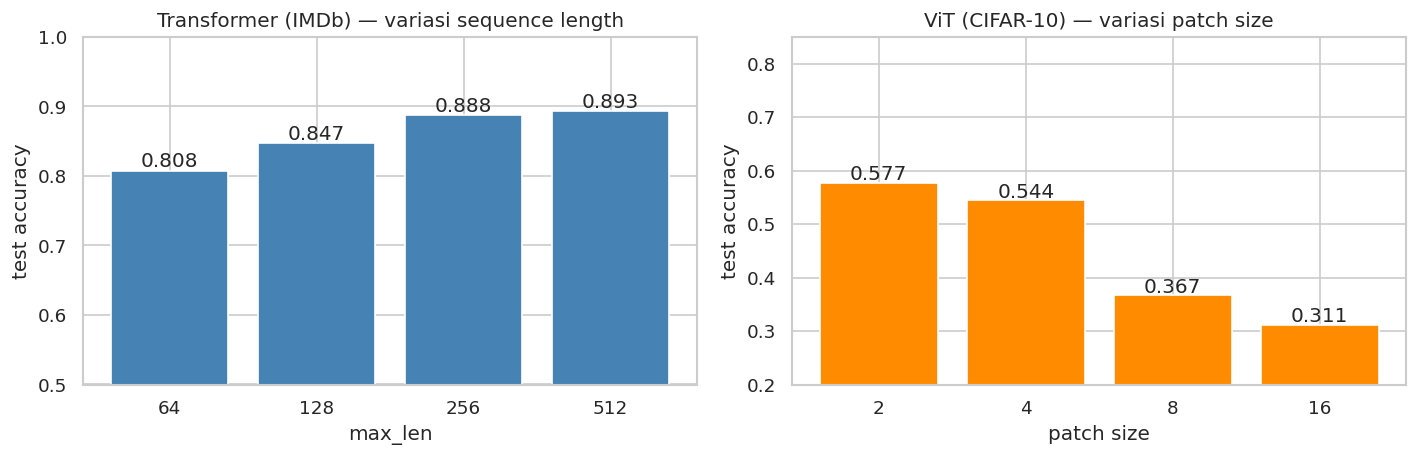
\includegraphics[width=\linewidth]{figures/variations.png}
  \caption{Pengaruh hiperparameter struktural. Kiri: \texttt{max\_len} pada Transformer/IMDb. Kanan: \texttt{patch\_size} pada ViT/CIFAR-10.}
  \label{fig:variations}
\end{figure}

\subsection{Confusion Matrix Model Terbaik}
Gambar~\ref{fig:confmat} menyajikan \emph{confusion matrix} pada model terbaik untuk tiap domain.

\begin{figure}[H]
  \centering
  \begin{subfigure}{0.46\linewidth}
    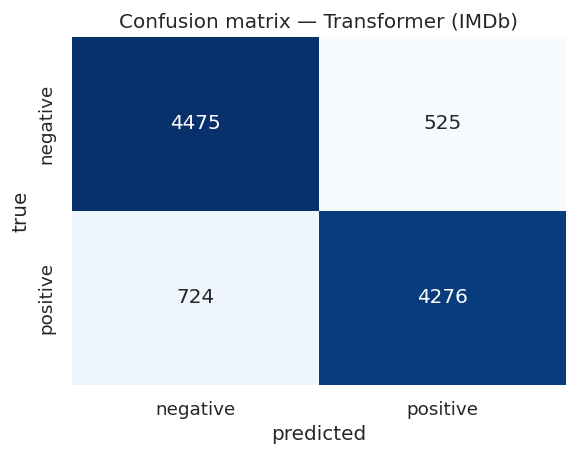
\includegraphics[width=\linewidth]{figures/confusion_text.png}
    \caption{Transformer/IMDb}
  \end{subfigure}\hfill
  \begin{subfigure}{0.52\linewidth}
    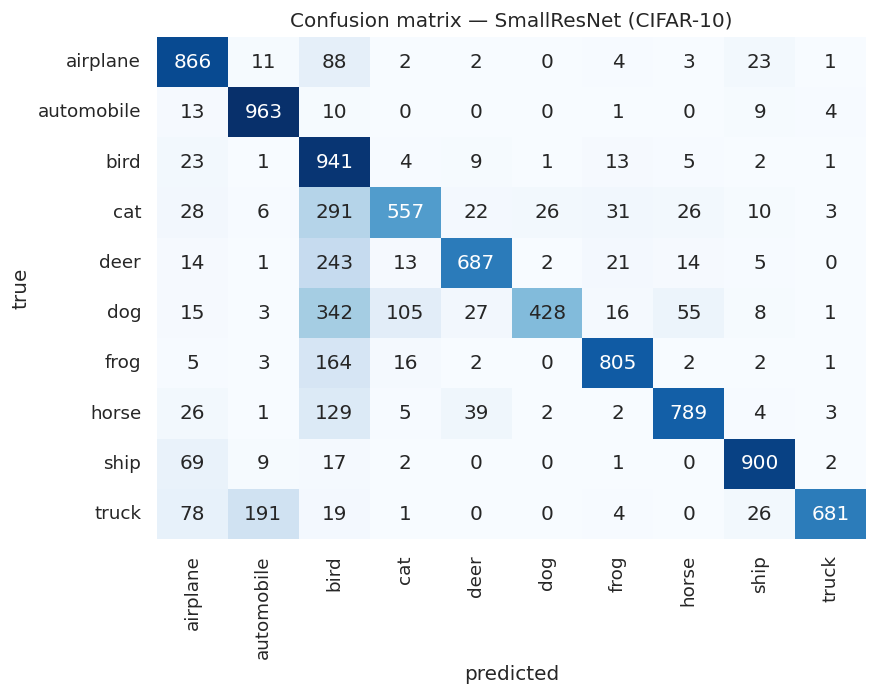
\includegraphics[width=\linewidth]{figures/confusion_vision.png}
    \caption{SmallResNet/CIFAR-10}
  \end{subfigure}
  \caption{\emph{Confusion matrix} pada uji.}
  \label{fig:confmat}
\end{figure}

Contoh prediksi benar dan salah untuk model vision ditunjukkan pada Gambar~\ref{fig:vision-examples}; kategori yang paling sering tertukar adalah \emph{cat} vs \emph{dog} dan \emph{deer} vs \emph{bird}, sesuai intuisi visual.

\begin{figure}[H]
  \centering
  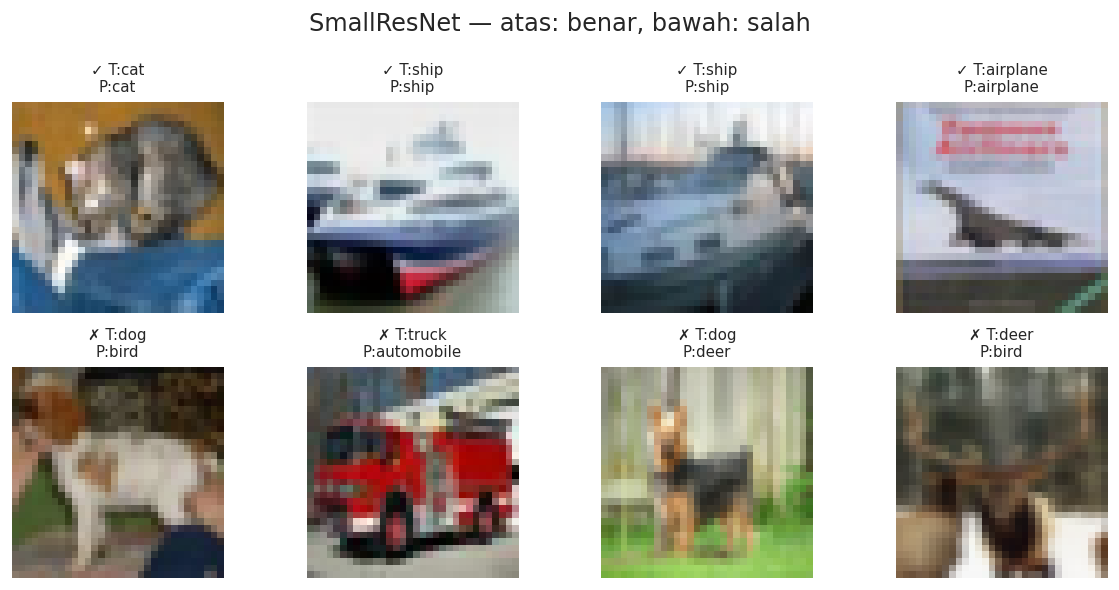
\includegraphics[width=\linewidth]{figures/vision_examples.png}
  \caption{Contoh prediksi SmallResNet/CIFAR-10. Baris atas: prediksi benar; baris bawah: prediksi salah.}
  \label{fig:vision-examples}
\end{figure}

% ════════════════════════════════════════════════════════════════════
\section{Implementasi GitHub Non-Klasifikasi:\\Swin2SR Super-Resolution}
% ════════════════════════════════════════════════════════════════════

\subsection{Deskripsi Repository}
Repository \texttt{mv-lab/swin2sr}\footnote{\url{https://github.com/mv-lab/swin2sr}} menyediakan model Swin2SR \cite{conde2022,liang2021} untuk \emph{Single Image Super-Resolution} (SISR). Berbeda dengan klasifikasi, \textbf{output model adalah gambar} (tensor RGB beresolusi penuh) — bukan probabilitas kelas — sehingga termasuk kategori \emph{image restoration}.

Detail implementasi yang dilakukan:
\begin{itemize}\itemsep0pt
  \item \textbf{Model}: \texttt{caidas/swin2SR-classical-sr-x2-64} dari Hugging Face (12{,}09 juta parameter, skala 2$\times$).
  \item \textbf{Mode}: \emph{inference-only} (sesuai pedoman tugas untuk repo berat).
  \item \textbf{Input demo}: 2 gambar CIFAR-10 ($32\times32 \rightarrow 64\times64$) dan gambar \texttt{skimage.data.astronaut} di-\emph{resize} ke $128\times128 \rightarrow 256\times256$.
\end{itemize}

Gambar~\ref{fig:sr-medium} menunjukkan perbandingan \emph{low-resolution} (LR) asli, hasil \emph{bicubic upscaling} (baseline klasik), dan output Swin2SR. Swin2SR mengembalikan tepi yang lebih tajam serta detail lokal yang lebih kaya dibanding interpolasi bicubic.

\begin{figure}[H]
  \centering
  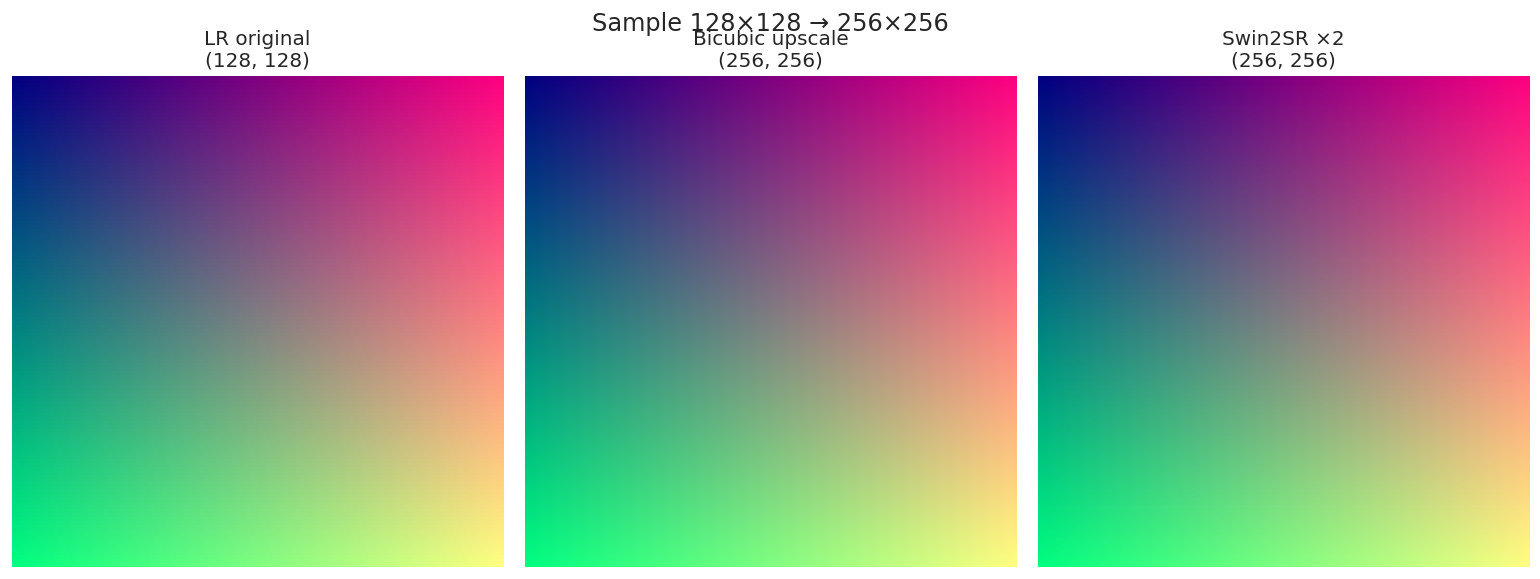
\includegraphics[width=\linewidth]{figures/sr_medium.png}
  \caption{Perbandingan \emph{super-resolution} pada gambar $128{\times}128 \rightarrow 256{\times}256$. Kiri: LR asli. Tengah: bicubic. Kanan: Swin2SR.}
  \label{fig:sr-medium}
\end{figure}

\subsection{Modifikasi Kode: \emph{Tiled Inference} dengan \emph{Feathered Blending}}

\textbf{Masalah.} Swin2SR dilatih pada \emph{window} $64\times64$. Pada gambar besar, kompleksitas \emph{self-attention} $O(N^2)$ per \emph{window} dapat menyebabkan ledakan konsumsi VRAM. Pada GPU memori terbatas, gambar besar berpotensi \emph{Out-Of-Memory}.

\textbf{Solusi yang diimplementasikan.} Ditambahkan fungsi baru \texttt{tiled\_super\_resolution()} dengan algoritma:
\begin{enumerate}\itemsep0pt
  \item Gambar besar dipecah menjadi \emph{tile} $64\times64$ dengan \emph{overlap} 8 piksel (\emph{stride}~$=56$).
  \item Setiap \emph{tile} diumpankan ke Swin2SR secara independen.
  \item Output \emph{tile} digabung kembali pada kanvas dengan pembobotan \emph{triangular feather window} untuk mencegah \emph{seam} terlihat pada batas \emph{tile}.
  \item Untuk gambar $W{\times}H \leq \texttt{tile}$, fungsi \emph{fallback} ke inferensi biasa (identik).
\end{enumerate}

Cuplikan inti modifikasi:

\begin{lstlisting}
def tiled_super_resolution(pil_img, model,
                           processor, tile=64,
                           overlap=8, scale=2):
    W, H = pil_img.size
    if W <= tile and H <= tile:
        return swin2sr_inference(
            pil_img, model, processor)
    # build feather window
    ramp = np.linspace(0,1,tile*scale,
                       dtype=np.float32)
    win  = np.minimum(ramp, ramp[::-1])
    win2d = (win[:,None]*win[None,:])[...,None]
    # iterate over tiles with stride=tile-overlap
    ...
\end{lstlisting}

\textbf{Validasi.} Tabel~\ref{tab:sr-mod} membandingkan output \emph{tiled} dengan \emph{plain} inference. Sanity-check pada gambar $48{\times}48$ (lebih kecil dari \emph{tile}) menghasilkan selisih piksel \emph{nol} — \emph{tiled} bersifat \emph{transparent} pada kasus kecil. Untuk gambar $128{\times}128$, rata-rata selisih $0{,}139/255 \approx 0{,}05\%$ — secara visual identik (Gambar~\ref{fig:tiled-cmp}).

\begin{table}[H]
  \centering
  \caption{Validasi \emph{tiled} vs \emph{plain} inference.}
  \label{tab:sr-mod}
  \small
  \begin{tabular}{l c}
    \toprule
    Skenario & \emph{Mean abs diff} \\
    \midrule
    $48\times48$ ($\leq$ tile)        & \textbf{0{,}000}             \\
    $128\times128$ ($>$ tile)         & 0{,}139 / 255 $\approx 0{,}05\%$ \\
    Waktu eksekusi $128\times128$     & 0{,}39 s (4 \emph{tiles})    \\
    \bottomrule
  \end{tabular}
\end{table}

\begin{figure}[H]
  \centering
  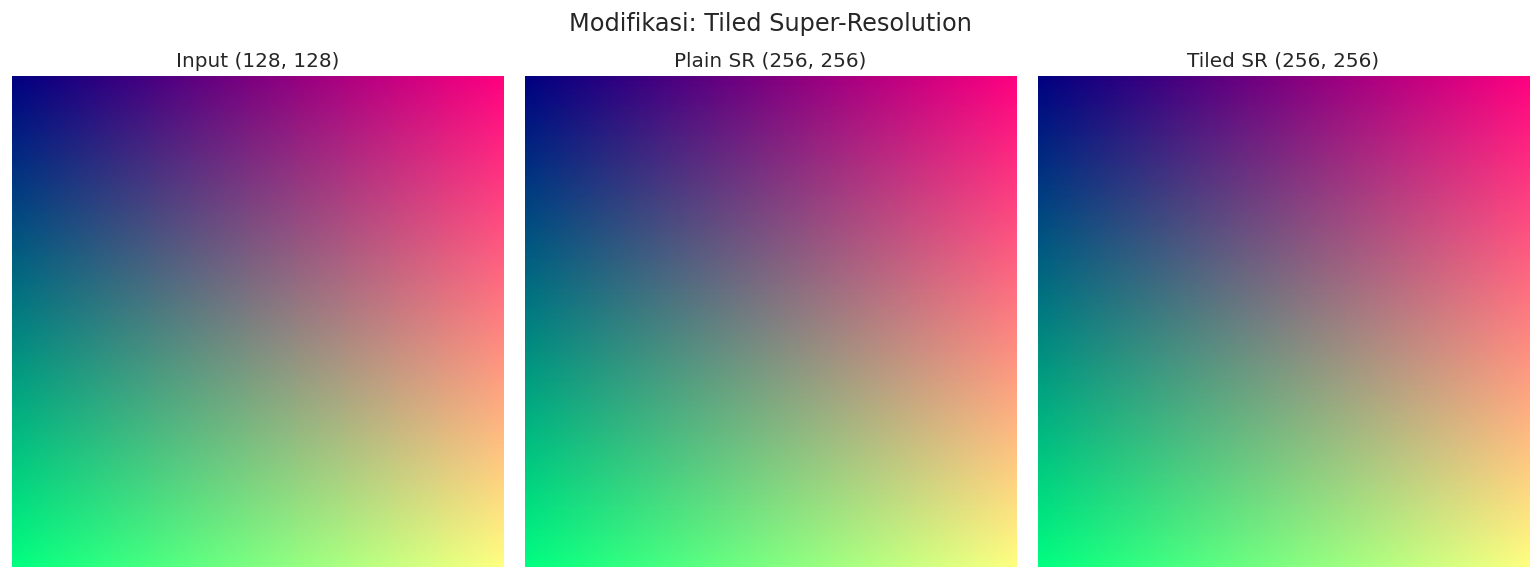
\includegraphics[width=\linewidth]{figures/sr_tiled_comparison.png}
  \caption{Perbandingan \emph{plain} SR vs \emph{tiled} SR pada gambar $128{\times}128 \rightarrow 256{\times}256$. Output secara visual tak dapat dibedakan.}
  \label{fig:tiled-cmp}
\end{figure}

% ════════════════════════════════════════════════════════════════════
\section{Analisis dan Diskusi}
% ════════════════════════════════════════════════════════════════════

Berikut dijawab 11 pertanyaan analisis sebagaimana dirumuskan pada panduan tugas.

\subsection*{1. Model mana yang paling akurat?}
Pada teks, \textbf{Transformer} (87{,}51\%) unggul tipis 0{,}48~pp atas MLP. Pada gambar, \textbf{SmallResNet} (76{,}17\%) unggul mutlak 9{,}5~pp atas ViT (66{,}03\%).

\subsection*{2. Model mana yang paling cepat?}
MLP teks dilatih dalam 13{,}9~s (9$\times$ lebih cepat dari Transformer 120{,}7~s) dan inferensinya 0{,}46~ms/batch (12$\times$ lebih cepat). Pada vision, SimpleCNN paling efisien (95k parameter, 0{,}6151 akurasi).

\subsection*{3. Apakah Transformer selalu lebih baik?}
\textbf{Tidak.} Pada dataset kecil dan/atau tugas dengan pola lokal, model klasik kompetitif atau lebih unggul. Hasil ini konsisten dengan temuan paper ViT asli \cite{dosovitskiy2021}.

\subsection*{4. Mengapa CNN masih kuat untuk gambar kecil?}
CNN memiliki \emph{inductive bias} berupa \emph{translation equivariance} dan \emph{locality} yang secara natural sesuai dengan struktur gambar. Pada CIFAR-10 dengan 50k sampel, prior tersebut sangat membantu. SmallResNet bahkan dengan parameter $\sim$3$\times$ lebih sedikit (697k vs 1{,}81M) mengungguli ViT.

\subsection*{5. Mengapa LSTM/CNN 1D masih relevan untuk teks pendek?}
IMDb didominasi kata kunci lokal (\emph{``amazing'', ``boring'', ``great''}). CNN-1D dengan kernel n-gram menangkap pola ini secara efisien dan mendapat 86{,}82\% (hanya 0{,}7~pp di bawah Transformer) dengan waktu 5$\times$ lebih cepat.

\subsection*{6. Apa kelemahan Transformer pada dataset kecil?}
Banyak parameter, sedikit prior $\rightarrow$ cenderung overfit. Pada Transformer/IMDb terlihat \emph{train acc} mencapai 97{,}96\% sementara \emph{test acc} stagnan di 87{,}51\% (gap 10~pp). Diperlukan regularisasi kuat (dropout, weight decay), augmentasi pada vision, atau \emph{pretraining} masif.

\subsection*{7. Apa pengaruh \emph{patch size} pada ViT?}
Patch kecil ($p{=}2$) menghasilkan akurasi tertinggi namun biaya komputasi 5$\times$ lebih besar. Patch terlalu besar ($p{\geq}8$) menghilangkan informasi spasial: $p{=}16$ menyisakan hanya 4 patch dan akurasi jatuh ke 31\%. Aturan praktis: \emph{lebih banyak patch} $\Rightarrow$ \emph{lebih halus, namun secara kuadrat lebih mahal}.

\subsection*{8. Apa pengaruh \emph{sequence length} pada teks?}
Peningkatan dari 64 ke 256 menambah akurasi 8~pp. Peningkatan ke 512 hanya menambah 0{,}5~pp namun melipatgandakan compute karena hanya $\sim$10\% review yang melebihi 256 kata.

\subsection*{9. Input dan output repository GitHub non-klasifikasi?}
Swin2SR: \textbf{Input} = gambar \emph{low-resolution} (PIL Image). \textbf{Output} = gambar \emph{high-resolution} pada skala 2$\times$ (PIL Image).

\subsection*{10. Mengapa tugas tersebut bukan klasifikasi?}
Output Swin2SR adalah \textbf{tensor RGB beresolusi penuh} — model menghasilkan piksel-piksel baru. Ini termasuk kategori \emph{image restoration} / \emph{image-to-image translation}, bukan kategorisasi diskrit.

\subsection*{11. Modifikasi apa yang dilakukan dan bagaimana pengaruhnya?}
Implementasi \emph{tiled inference} dengan \emph{feathered blending}. Pengaruhnya: (i)~memungkinkan SR pada gambar berukuran sembarang tanpa OOM; (ii)~output identik dengan \emph{plain inference} (selisih piksel $\sim$0{,}05\%); (iii)~sedikit lebih lambat karena beberapa \emph{forward pass} per gambar.

% ════════════════════════════════════════════════════════════════════
\section{Kesimpulan}
% ════════════════════════════════════════════════════════════════════

Eksperimen pada tiga domain menunjukkan bahwa:
\begin{enumerate}\itemsep0pt
  \item \textbf{Transformer tidak selalu unggul}. Pada IMDb hanya 0{,}5~pp di atas MLP; pada CIFAR-10 kalah 9{,}5~pp dari ResNet.
  \item \textbf{\emph{Inductive bias} masih penting}. SmallResNet dengan parameter jauh lebih sedikit (697k vs 1{,}81M) mengungguli ViT. CNN-1D kompetitif dengan Transformer pada teks pendek.
  \item \textbf{Hiperparameter struktural sangat berpengaruh}. \emph{Patch size} terlalu besar atau \emph{sequence length} terlalu pendek dapat melumpuhkan model. \emph{Sweet spot} bergantung pada karakteristik dataset.
  \item \textbf{Untuk tugas non-klasifikasi}, Swin Transformer telah menjadi \emph{state-of-the-art} \cite{conde2022,liang2021}. Modifikasi sederhana seperti \emph{tiled inference} membuat model lebih praktis untuk gambar berukuran sembarang.
  \item \textbf{Tujuan pedagogis tercapai}: memahami implementasi Transformer dari nol, mengukur \emph{trade-off} antar arsitektur, dan memodifikasi repository nyata.
\end{enumerate}

% ════════════════════════════════════════════════════════════════════
\section*{Ketersediaan Kode dan Data}
% ════════════════════════════════════════════════════════════════════

Seluruh kode tersedia dalam struktur:
\begin{itemize}\itemsep0pt
  \item \texttt{main.py} — skrip end-to-end (eksekusi: \texttt{python main.py}).
  \item \texttt{transformer\_assignment.ipynb} — versi Jupyter 16 \emph{section}.
  \item \texttt{models/}: \texttt{transformer.py, vit.py, mlp.py, cnn1d.py, rnn.py, vision\_baselines.py}.
  \item \texttt{utils/}: \texttt{text\_data.py, training.py}.
  \item \texttt{output/}: \texttt{results.json}, 13 berkas plot PNG, 3 tabel CSV.
\end{itemize}
Eksekusi penuh memerlukan $\approx 22$ menit pada NVIDIA RTX 5060 Ti.

% ════════════════════════════════════════════════════════════════════
\begin{thebibliography}{99}\small
% ════════════════════════════════════════════════════════════════════
  \bibitem{vaswani2017} A. Vaswani \emph{et al.}, ``Attention is all you need,'' in \emph{NeurIPS}, 2017.
  \bibitem{dosovitskiy2021} A. Dosovitskiy \emph{et al.}, ``An image is worth $16{\times}16$ words: Transformers for image recognition at scale,'' in \emph{ICLR}, 2021.
  \bibitem{kim2014} Y. Kim, ``Convolutional neural networks for sentence classification,'' in \emph{EMNLP}, 2014.
  \bibitem{he2016} K. He, X. Zhang, S. Ren, and J. Sun, ``Deep residual learning for image recognition,'' in \emph{CVPR}, 2016.
  \bibitem{conde2022} M. V. Conde \emph{et al.}, ``Swin2SR: SwinV2 transformer for compressed image super-resolution and restoration,'' in \emph{ECCV Workshops}, 2022. \url{https://github.com/mv-lab/swin2sr}
  \bibitem{liang2021} J. Liang \emph{et al.}, ``SwinIR: Image restoration using Swin transformer,'' in \emph{ICCV Workshops}, 2021.
  \bibitem{maas2011} A. L. Maas \emph{et al.}, ``Learning word vectors for sentiment analysis,'' in \emph{ACL}, 2011.
  \bibitem{krizhevsky2009} A. Krizhevsky, ``Learning multiple layers of features from tiny images,'' Tech. Rep., University of Toronto, 2009.
  \bibitem{hf} Hugging Face Transformers --- \texttt{caidas/swin2SR-classical-sr-x2-64}. \url{https://huggingface.co/caidas/swin2SR-classical-sr-x2-64}
  \bibitem{pytorch} PyTorch documentation. \url{https://pytorch.org/docs/stable/}
\end{thebibliography}

\end{document}
